%% LaTeX-Beamer template for KIT design
%% by Erik Burger, Christian Hammer
%% title picture by Klaus Krogmann
%%
%% version 2.1
%%
%% mostly compatible to KIT corporate design v2.0
%% http://intranet.kit.edu/gestaltungsrichtlinien.php
%%
%% Problems, bugs and comments to
%% burger@kit.edu

\documentclass[18pt]{beamer}

%% SLIDE FORMAT

% use 'beamerthemekit' for standard 4:3 ratio
% for widescreen slides (16:9), use 'beamerthemekitwide'

\usepackage{templates/beamerthemekit}
%\usepackage{templates/beamerthemekitwide}

\usepackage[utf8]{inputenc}

%% TITLE PICTURE

% if a custom picture is to be used on the title page, copy it into the 'logos'
% directory, in the line below, replace 'mypicture' with the 
% filename (without extension) and uncomment the following line
% (picture proportions: 63 : 20 for standard, 169 : 40 for wide
% *.eps format if you use latex+dvips+ps2pdf, 
% *.jpg/*.png/*.pdf if you use pdflatex)

\titleimage{btw_titel}

%% TITLE LOGO

% for a custom logo on the front page, copy your file into the 'logos'
% directory, insert the filename in the line below and uncomment it

%\titlelogo{mylogo}

% (*.eps format if you use latex+dvips+ps2pdf,
% *.jpg/*.png/*.pdf if you use pdflatex)

%% TikZ INTEGRATION

% use these packages for PCM symbols and UML classes
% \usepackage{templates/tikzkit}
% \usepackage{templates/tikzuml}

% the presentation starts here

\title[Qualitätssicherungsphase]{OpenBundestagswahl}
\subtitle{Qualitätssicherungsphase}
\author{Simon Schürg}

\institute{Praxis der Softwareentwicklung, WS 2013/14}

% Bibliography

\usepackage[citestyle=authoryear,bibstyle=numeric,hyperref,backend=biber]{biblatex}
%\addbibresource{templates/example.bib}
\bibhang1em

\begin{document}

% change the following line to "ngerman" for German style date and logos
%\selectlanguage{english}
\selectlanguage{ngerman}

%title page
\begin{frame}
\titlepage
\end{frame}

%table of contents
\begin{frame}{Gliederung}
\tableofcontents
\end{frame}


\section{Modultests}
\begin{frame}{Modultests}
\begin{itemize}
	\item Regressionstests mittels \textbf{JUnit}
	\begin{itemize}
		\item Zum automatischen und wiederholbaren Testen
		\item Nur für Module der Anwendungslogik
	\end{itemize}
	\item Codeanalyse mit \textbf{FindBugs}
	\begin{itemize}
		\item Untersuchung von Code auf bekannte Fehlermuster
	\end{itemize}
	\item Organisation mit \textbf{Redmine} Ticketsystem\\
\end{itemize}
\end{frame}

\subsection{Mandatsrechner}
\begin{frame}{Mandatsrechner}
\begin{itemize}
	\item Kern-Feature der Anwendung
	\item Korrekte Berechnung gemäß Wahlgesetz sehr wichtig
	\item Viele Spezialfälle und Zufall (Auslosen) macht Testen aufwändig
	\item Probleme mit Endlosschleifen
\end{itemize}
\end{frame}

\subsection{Model}
\begin{frame}{Model}
\begin{itemize}
	\item Komplexe Objektstruktur des Models macht Testen aufwändig
	\begin{itemize}
		\item Viele Ausnahmen müssen überprüft werden
		\item Konsistenz der Datenobjekte muss gewährleistet sein (Anforderung aus dem Pflichtenheft)
	\end{itemize}
	
\end{itemize}
\end{frame}

\subsection{Wahlgenerator}
\begin{frame}{Wahlgenerator}
\begin{itemize}
	\item Generierung nur mit gültigen Stimmanteilen
	\item Erzeugen einer Wahl muss mit gültigen Parametern immer möglich sein
	\item Probleme mit Wahlkreisen ohne Stimmen
\end{itemize}
\end{frame}

\subsection{Wahlvergleich}
\begin{frame}{Wahlvergleich}
\begin{itemize}
	\item Berechnung der Differenzen muss stimmen
\end{itemize}
\end{frame}

\subsection{Import/Export und Config}
\begin{frame}{Import/Export und Config}
\begin{itemize}
	\item Prüfen von CSV-Dateien auf Gültigkeit
	\item Alle relevanten Informationen korrekt einlesen und wieder schreiben
	\item Probleme mit unterschiedlichen Zeichensätzen
\end{itemize}
\end{frame}

\subsection{Testabdeckung}
\begin{frame}{Testabdeckung}
\begin{itemize}
	\item EclEmma zur automatischen Überprüfung der Testabdeckung
	\item Methoden gefunden die nicht benötigt wurden
	\item Methoden gefunden deren Funktionalität doppelt vorhanden war
\end{itemize}
\end{frame}

\begin{frame}{EclEmma}
\begin{itemize}
	\item Anweisungsübderdeckung\\
	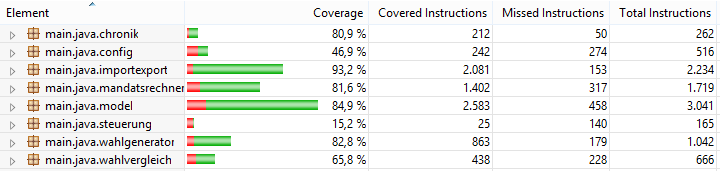
\includegraphics[scale=0.4]{img/anweisungsueberdeckung.png}
	\item Zweigüberdeckung
	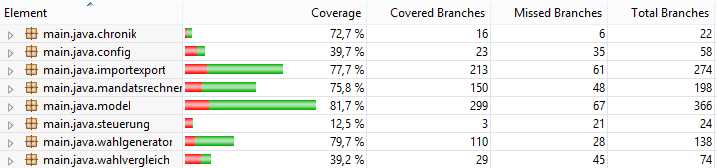
\includegraphics[scale=0.4]{img/zweigueberdeckung.png}
\end{itemize}
\end{frame}


\section{Integrations- und Systemtests}
\begin{frame}{Integrations- und Systemtests}
\begin{itemize}
	\item Manuell durchgeführte Tests
	\item Anforderungen aus dem Pflichtenheft
	\begin{itemize}
		\item Nicht-funktionale Anforderungen
		\item Laufzeit, Bedienbarkeit \dots
	\end{itemize}
\end{itemize}
\end{frame}

\subsection{GUI}
\begin{frame}{GUI}
\begin{itemize}
	\item GUI wurde manuell getestet
	\item Unterschiedliche Probleme wurden behoben
	\begin{itemize}
		\item Layout
		\item Oberflächenlogik
		\item Fehlerbehandlung und Meldungen
	\end{itemize}
\end{itemize}
\end{frame}

\begin{frame}{GUI}
\begin{itemize}
	\item Performance Probleme
	\item Analyse mit JVisualVM war sehr hilfreich\\
	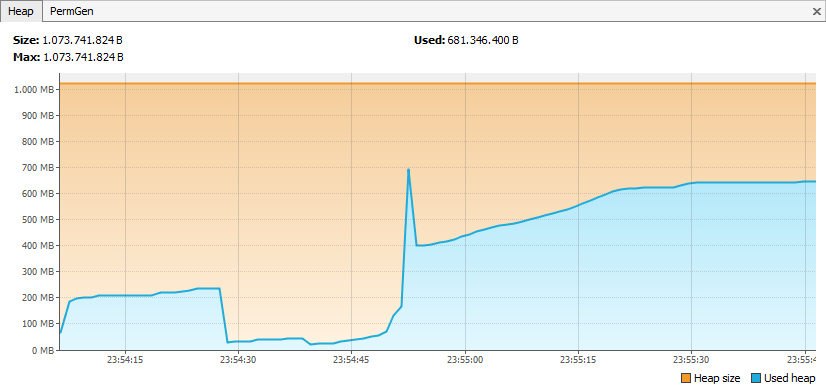
\includegraphics[scale=0.2]{img/mitFehler.png}\\
	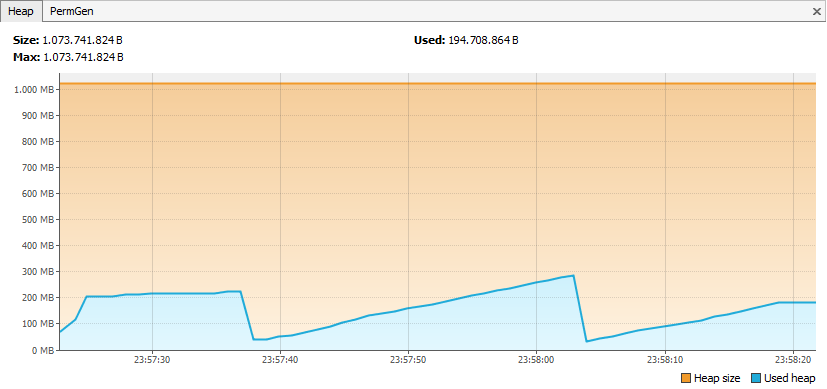
\includegraphics[scale=0.2]{img/ohneFehler.png}
\end{itemize}
\end{frame}

\subsection{Plattformunabhängigkeit}
\begin{frame}{Plattformunabhängigkeit}
\begin{itemize}
	\item Unter Windows entwickelt
	\item Unter Windows und Linux getestet und lauffähig\\
	\begin{center}
		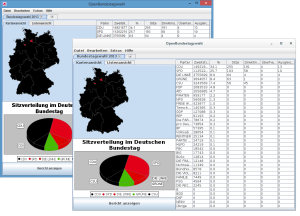
\includegraphics[scale=0.7]{img/app_klein.png}
	\end{center}
\end{itemize}
\end{frame}

\section{Veränderungen und Sonstiges}
\begin{frame}{Veränderungen}
\begin{itemize}
	\item Simulation des negativen Stimmgewichts entfernt
	\item Hilfe Dialoge verwenden keine JavaFX Webviews mehr
	\item Handbuch wurde neu geschrieben
	\item Zusätzliche Features
	\begin{itemize}
		\item Sortierung der Tabellen
		\item Debug Klasse
	\end{itemize}
	\item Name der Anwendung ist \textbf{OpenBundestagswahl}
\end{itemize}
\end{frame}

\section{Fazit}
\begin{frame}{Fazit}
\begin{itemize}
	\item Es konnten viele Fehler gefunden und behoben werden
	\item Wir sind mit der Qualität der Software zufrieden
	\item Automatische Regressionstests sind uns wichtiger geworden
	\begin{itemize}
		\item Wäre auch schon in der Implementierungsphase sinnvoll gewesen
	\end{itemize}
	
\end{itemize}
\end{frame}

\section{Ausblick}
\begin{frame}{Ausblick}
\begin{itemize}
	\item Entwicklung ist abgeschlossen
	\item In den letzten beiden Projektwochen ist Manuel Olk Phasenverantwortlicher
\end{itemize}
\end{frame}


\appendix

\begin{frame}{}

\begin{LARGE}
\begin{center}
	Vielen Dank für Ihre Aufmerksamkeit!
\end{center}
\end{LARGE}
\end{frame}

\end{document}
